\chapter{Loop Closure}
\label{chapter:loop_closure}

Dieses Kapitel beschäftigt sich mit der Detektion von Schleifenschlüssen und der damit verbundenen Optimierung der initialen Schätzung einer Trajektorie beziehungsweise eines Pose-Graphen, entlang dessen ein Sensorsystem bewegt wurde. Im Folgenden wird zunächst näher auf den Detektionsschritt eingegangen. Auf Basis dessen wird in den drauf folgenden Abschnitten die in dieser Arbeit verwendete Methode zur Optimierung des Pose-Graphen eruiert.

\section{Detektion}

Dieser Abschnitt befasst sich mit der Detektion von Schleifenschlüssen in einem Pose-Graphen. Die hier vorgestellte Methode kann sowohl in einem inkrementell erweiterten Pose-Grahen, zum Beispiel als zusätzlicher Schritt in einem SLAM Verfahren, als auch in einem Nachbearbeitungsschritt auf einen bereits fertigen Graphen angewandt werden. Die Methode und die Optimierung des Graphen ist dabei zunächst vollständig losgelöst von der TSDF-Karte, die im Anschluss optimiert wird. Mehr dazu in Kapitel \ref{chapter:map_update}. 

Bevor nach Schleifenschlüssen gesucht werden kann, gilt es zu bestimmen, von welcher Pose aus gesucht werden soll. In einem inkrementellen SLAM Verfahren wäre das jeweils die aktuell betrachtete, zuletzt in den Graphen eingefügte Pose. In einem Nachbearbeitungsschritt wird dieser inkrementelle Prozess imitiert, indem der Pose-Graph, beginnend von der ersten eingefügten Pose, abgelaufen wird. In beiden Fällen wird also ein Schleifenschluss mit Posen gesucht, die früher in den Graphen eingefügt wurden als die aktuelle Pose $P_{cur}$. In einem ersten Schritt wird hierzu eine Menge von Schleifenschluss-Kandidaten erstellt. Diese Menge ergibt sich aus der in \cite{borrmann2008globally, shan2020lio} vorgestellten euklidischen Distanzmetrik, die in dieser Arbeit verwendet wird. Eine Pose $P_i$ gilt als Schleifenschluss-Kandidat zu $P_{cur}$, wenn die euklidische Distanz zwischen den beiden Posen geringer ist als eine parametrisierbare Schwelle $d_{max}$. Zusätzlich zu diesem Parameter wird an dieser Stelle ein weiterer Parameter $d_{trav}$ eingeführt der die minimale Distanz definiert, die der Sensorsystem entlang des Teilpfades gegeben durch $P_i$ und $P_{cur}$ zurückgelegt hat. Um Posen zu identifizieren, die diese Voraussetzungen Erfüllen, wird ein \textbf{k-d tree (k-d Baum)} \cite{bentley1975multidimensional} verwendet. Ein k-d Baum ist eine Datenstruktur zur Speicherung von (räumlichen) Informationen, die durch assoziative Suchen abgefragt werden können. Ein k-d Baum eignet sich aufgrund der optimierten Laufzeit besonders für räumliche Suchen. Dabei steht das \textbf{k} für die Dimensionalität des Suchraums \cite{bentley1975multidimensional}. An dieser Stelle wird der k-d Baum zur Speicherung von \textbf{3-d} Daten genutzt. Diese ergeben sich aus den Posen des Pfades. Vor jeder Detektion wird ein neuer k-d Baum aus den Translationsanteilen aller zuvor eingefügten Posen aufgebaut. Im Anschluss wird eine Radius-Suche durchgeführt, die alle Daten des k-d Baumes (hier 3-d Punkte) zurückliefert, deren euklidische Distanz zu einer übergebenen Position geringer ist als eine übergebene Schwelle. Die übergebene Position ist dabei der Translationsanteil von $P_cur$ und die übergebene Schwelle $d_max$. Ergebnis ist eine Menge von Kandidaten für Schleifenschlüsse $\mathbb{K} = \left\lbrace K_0, ..., K_k \right\rbrace$. Diese Arbeit verwendet die k-d Baum Implementation der \textbf{Pointcloud Library (PCL)} \ref{rusu20113d}.

Über die generierten Kandidaten ist an dieser Stelle lediglich bekannt, dass sie sich im nicht optimierten Pfad in der Nähe der aktuellen Pose $P_{cur}$ befinden. Diese räumliche Nähe ist an dieser Stelle allerdings nur eine Annahme, die es zu verifizieren gilt. Als Basis für die Verifikation dient die in diesem Ansatz gegebene Datenbasis in Form von zu jeder Pose des Pose-Graphen $\mathfrak{P}_{init} = \left\lbrace P_0, ..., _n \right\rbrace$ zugehörigen Punktwolken $ \mathbb{C} = \left\lbrace C_0, ..., C_n \right\rbrace$. Für die aktuell betrachte Pose $P_{cur}$ und die zugehörige Punktwolke wird ein Scan-Matching gegen jeden Kandidaten aus  $\mathbb{K}$ und dessen zugehörigen Punktwolken $C_i$ durchgeführt und evaluiert. Konvergiert das Scan-Matching mit einer festgelegten Genauigkeit ist der Kandidat validiert. Im Folgenden wird die Punktwolke der aktuell betrachteten Pose $P_{cur}$ als Scan-Punktwolke $C_{scan}$ und die zum zu validierenden Kandidaten zugehörige Punktwolke als Model-Punktwolke $C_{model}$ bezeichnet. Grundlage für das Scan-Matching der beiden Punktwolken ist ein Algorithmus wie \textbf{ICP}, \textbf{GICP} oder vergleichbare Algorithmen zur Registrierung von Punktwolken. Diese Algorithmen liefern neben einer Information zur Konvergenz in der Regel zusätzlich ein Maß dafür zurück, wie gut die Punktwolken nach der Registrierung aufeinander passen. In dieser Arbeit werden hierzu die Implementationen der Algorithmen der Pointcloud Library \cite{rusu20113d} verwendet. Diese liefern für beide Algorithmen einen \textbf{Fitness-Score ($\Gamma$)} zurück, der die durchschnittliche quadrierte Distanz zwischen einem Punkt der Scan-Punktwolke und dem euklidisch nächste Punkt der Model-Punktwolke nach Registrierung der Scan-Punktwolke an die Model-Punktwolke beschreibt. Nachfolgende Formel zeigt diesen Sachverhalt mit $s_i$ als aktuellen Scanpunkt und $m_i$ als zugehörigen, euklidisch nächsten Punkt der Model-Punktwolke und $N$ als Anzahl der Punkte in der Scan-Punktwolke.

\begin{myequation}
\Gamma = \frac{\sum_{i = 0}^{N} \norm{\vec{m_i} - \vec{s_i}}^2}{N}
\end{myequation}

Liegt der Fitness-Score unter eine vordefinierten Schwelle $\Gamma_{max}$, ist der Kandidat validiert.
Zusätzlich liefern die Algorithmen die bestimmte finale Transformation $T_{fin}$ der Registrierung von Scan zu Model. Da GICP und ICP deutlich bessere Ergebnisse erzielen, wenn zwischen den Daten bereits eine Initialschätzung vorliegt, wird eine solche, auf Basis der jeweiligen Pose-Differenzen, genutzt. Die Punktwolkendaten liegen hier jeweils relativ zur Pose, von derer sie aufgenommen wurden, vor. Für die Initialschätzung wird nun die Model-Punktwolke ins Koordinatensystem der Scan-Punktwolke transformiert. Dazu wird zunächst die Transformation $T_{model \rightarrow scan}$ über die zugehörigen Posen $P_{model}$ und $P_{scan}$ und die zugehörigen Transformationen $T_{model \rightarrow map}$ und $T_{scan \rightarrow map}$ von den Posen ins Ursprungskoordinatensystem bestimmt:

\begin{myequation}
T_{model \rightarrow scan} = T_{scan \rightarrow map}^{-1} \cdot T_{model \rightarrow map}
\end{myequation}

Im Anschluss wird jeder Punkt $p_{model}^i$ der Punktwolke $C_{model}$ mit der bestimmten Transformation $T_{model \rightarrow scan}$ transformiert. Nun ist die Model-Punktwolke in das Koordinatensystem der Scan-Punktwolke, gegeben die aktuellen Pose-Schätzungen, vortransformiert. Diese Vortransformation muss nach der anschließenden Registrierung mittels ICP, GICP oder einem ähnlichen Verfahren für die Berechnung der finalen Transformation berücksichtigt werden. Dies ist in Abbildung \ref{fig:LoopIdentifikation} dargestellt. Sie führt zusätzlich die vom zur Registrierung berechneten Algorithmus bestimmte Transformation $T_{reg}$, sowie die sich daraus ergebene neue, approximative Pose $P_{scan}'$, von der die Scan-Punktwolke aufgenommen wurde. Die finale Transformation $T_{scan' \rightarrow model}$ die im weiteren Verlauf für die Optimierung des Pose-Graphen benötigt wird ergibt sich wie folgt:

\begin{myequation}
\label{math:final_transformation}
T_{scan' \rightarrow model} = T_{model \rightarrow scan}^{-1} \cdot T_{reg}
\end{myequation}

\begin{figure}
		\centering
		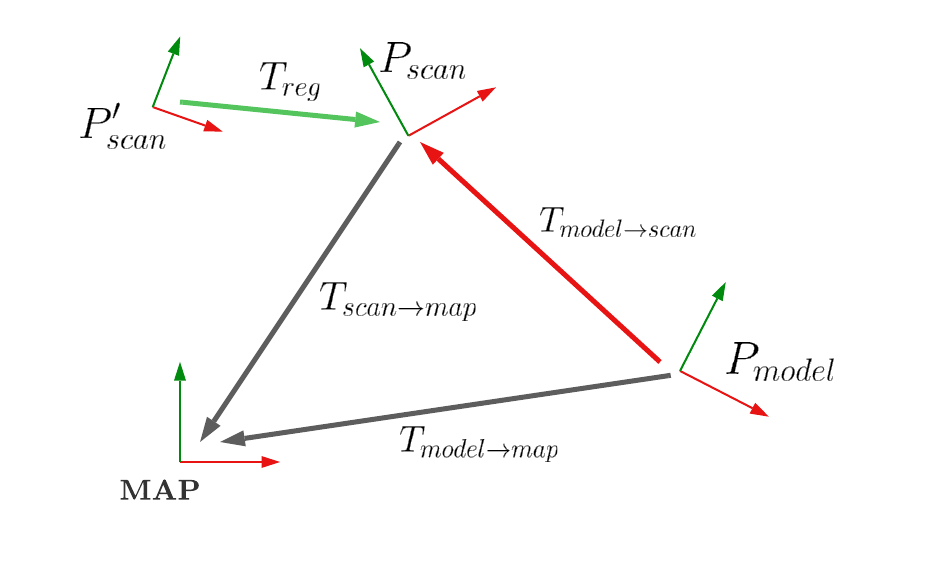
\includegraphics
			[scale=0.3]
			{LoopIdentifikation}
		\caption
			[Caption for LOF]{Diese Grafik stellt die Posen und Transformationen dar, die bei der Detektion eines Schleifenschlusses zur Verwendung kommen. Dabei bestimmt $T_{model \rightarrow scan}$ die Vortransformation vom lokalen Model-Koordinatensystem ins das des Scans (dargestellt in rot). In grün dargestellt ist die Transformation $T_reg$, die von dem verwendeten Algorithmus zur Registrierung der Scan-Punktwolke an die mit $T_{model \rightarrow scan}$ vortransformierte Model-Punktwolke, ausgegeben wird. Eine Kombination der Transformationen $T_reg$ und $T_{model \rightarrow scan}$ ergibt die finale, zur Optimierung des Pose-Graphen verwendete Transformationen. Diese Kombination ist in Gleichung \ref{math:final_transformation} definiert.}		                                                                                                                                     
		\label{fig:LoopIdentifikation}
\end{figure}

Auf diese Art und Weise können nur wenige Schleifenschlüsse identifiziert werden. Ursache ist zu diesem Zeitpunkt das Scan-Matching, welches zwar in den meisten Fällen konvergiert, jedoch fast keinen der Kandidaten aufgrund zu hoher Fitness-Scores validieren kann. Zusätzlich sind einige der identifizierten Schleifenschlüsse, besonders in Bereichen von Fluren oder Orten mit wenigen Features, fehlerhaft. Hier sind zwar die genannten Rahmenbedingungen erfüllt, allerdings verschlechtern die Schleifenschlüsse das Ergebnis maßgeblich.



Beschreibung der Detektion (bildhaft), Erklärung von Kandidaten und Filterung
Beschreibung des optionalen Sichtbarkeitskriteriums

\section{Graphenoptimierung}

Bezug zu GTSAM Library Beschreibung aufnehmen.
Wichtigste verwendete Funktionen bennen.
Verweis auf GTSAM Paper.
Erklärung von Faktorgraphen und Faktoren.
Erklärung der Genutzten datenstrukturen und optimizer.
Erklärung von noise constraints (Unsicherheiten)

\section{Optimierungen}

1. Vorregistrierung

2. Filtern der Punktwolke

3. Unterschiedliche Scan-Matching Varianten
	1. ICP
	2. GICP
	3. Kurz auf Teaser++ eingehen
	4. VGICP
	
	-> Analyse des Scan Matchings bezogen auf 1. Vorregistrierung, 2. LC Detektion Matching
	-> Graph über Fitness Counter mit LC Linie (dünn) verschiedene Farben
	-> dazu: starten mit allen varianten und jeweils werte akkumulieren
	-> schreiben in csv
	
	4. Rejectors
	
	\improvement{einführen: Pointcloud-Enrichment, Grafik: Fitness score im bezug zum enrichment: eine wolke vs. mehrere}

\section{Pseudocode}


\improvement{insert the pseudo code to the whole algorithm}
	
\section{Datensätze}

Verwendete Datensätze und herausforderungen herausstellen

\subsection{Hannover1}

Herausforderungen:

- Datensatz allgemein: falsches Koordindatensystem -> Transformation beschreiben

- extrem fehlerbehaftete Rotation in zweitem Kreis (Lösung: Vorregistrierung ICP)
(Scan-Matching bekommt extrem divergierte Wolken nicht mehr aufeinander)

- problematisch: fehlerhafte LC Optimierung durch schlechtes Scan Matching (Grund: Feature-armer Flur) -> mögliche ( noch zu entwickelnde) Lösung: LC's auf Linien gesondert betrachten -> Identifikation eines LC auf Linien -> Betrachtung der Scan Matching Transformation - wenn aufGeraden kann die Transformation die beiden LC-Punkte nicht vollständig zusammen ziehen

\subsection{Maps}

